\newpage
\section{Выполнение кассовых операций}

Основными функциями кассира в \tmisp~являются:

\begin{itemize}
 \item Прием и учет оплаты платных медицинских услуг;
 \item Заключение договоров на оказание платных услуг.
\end{itemize}

Для выполнения данных функций пользователю необходимо зайти в систему под ролью <<Кассир>>.


\subsection{Прием платежей}

Для выполнения функции приема платежей в \tmisp~нужно на панели навигации в левой части страницы щелкнуть по пиктограмме \dm{Прием платежей} или щелкнуть по плитке \dm{Прием платежей} на главной странице системы. Будет осуществлен переход на страницу \dm{Прием платежей} (Рисунок \ref{img_kas_mainpay}). 

\begin{figure}[ht]\centering
	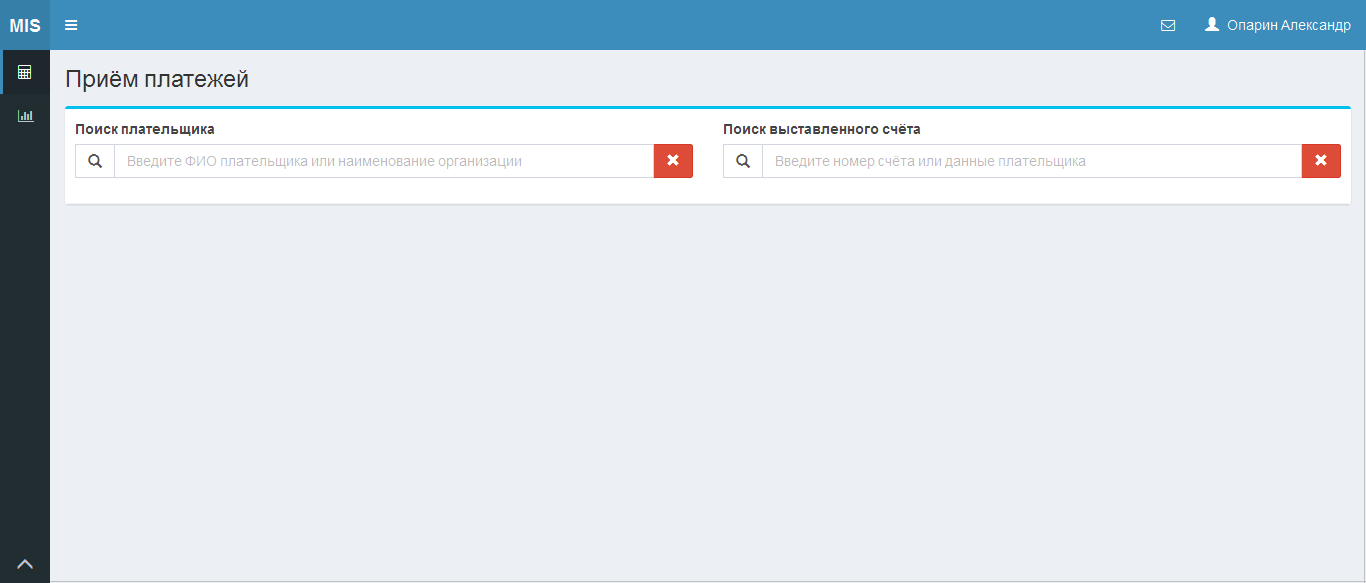
\includegraphics[width = 1\textwidth ,keepaspectratio]{kas_mainpay}
	\caption{Страница <<Прием платежей>>}
	\label{img_kas_mainpay}
\end{figure}

На данной странице возможен поиск:
\begin{itemize}
 \item По имени (наименованию) платильщика;
 \item По номеру счета на оплату медицинских услуг.
\end{itemize}

Для оплаты медицинских услуг по имени плательщика следует ввести фамилию плательщика (для физических лиц) или часть наименования организации (для юридических лиц) в поле \dm{Поиск плательщика}, расположенное в левом верхнем углу страницы. Поиск осуществляется автоматически по мере ввода текста в поле.

Как правило, в кассе осуществляется оплата набора медицинских услуг, сформированного в регистратуре. Такие наборы медицинских услуг называются счетами на оплату, имеют номер и дату формирования. Для поиска по номеру счета необходимо ввести его в поле \dm{Поиск выставленного счета}, расположенное в правом верхнем углу страницы.  Поиск осуществляется по мере ввода текста в поле.

По результатам поиска в нижней части страницы отобразится список счетов, найденных по заданным критериям поиска (Рисунок \ref{img_kas_getpay}). Для оплаченных счетов указана дата оплаты в поле \dm{Дата погашения}. Если счет не оплачен, то дата погашения для него пуста, но при этом доступна кнопка 
\includegraphics[scale=0.7]{payb} (Оплатить) в правой части строки.

\begin{figure}[ht]\centering
	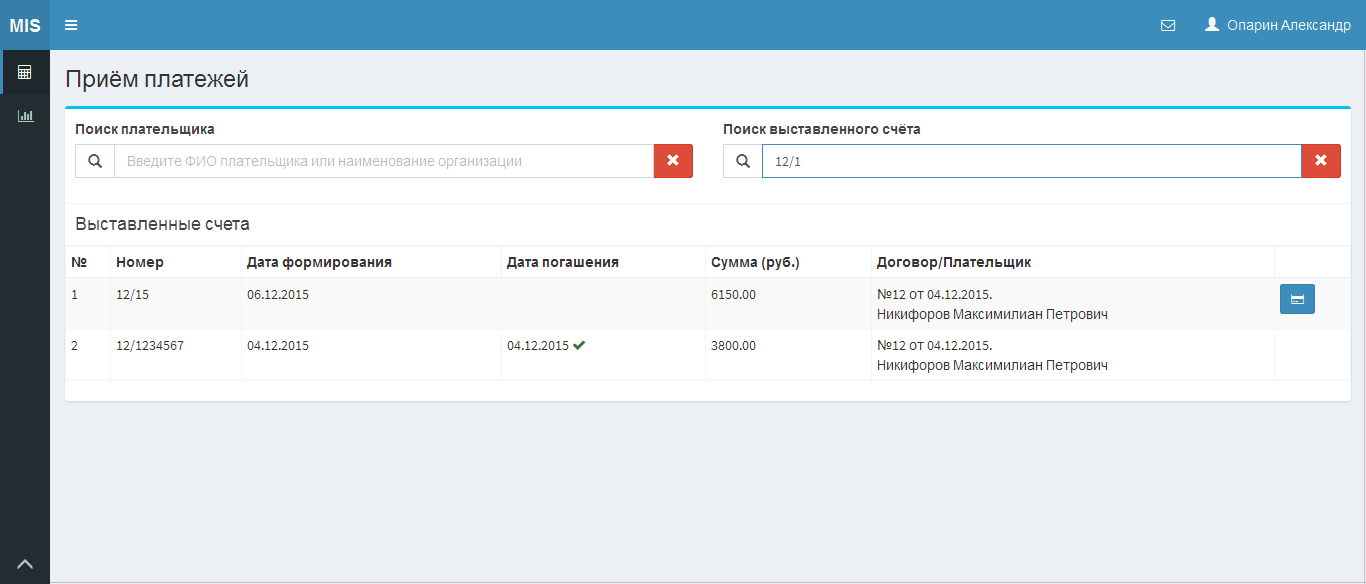
\includegraphics[width = 1\textwidth ,keepaspectratio]{kas_getpay}
	\caption{Страница <<Поиск счета по номеру>>}
	\label{img_kas_getpay}
\end{figure}

При нажатии на кнопку 
\includegraphics[scale=0.7]{payb} открывается всплывающее окно (Рисунок \ref{img_kas_payment}). В верхней части окна указывается номер и дата счета, имя(наименование) плательщика и сумма счета. В нижней части окна выводится перечень медицинских услуг, включенных в счет. 

\begin{figure}[ht]\centering
	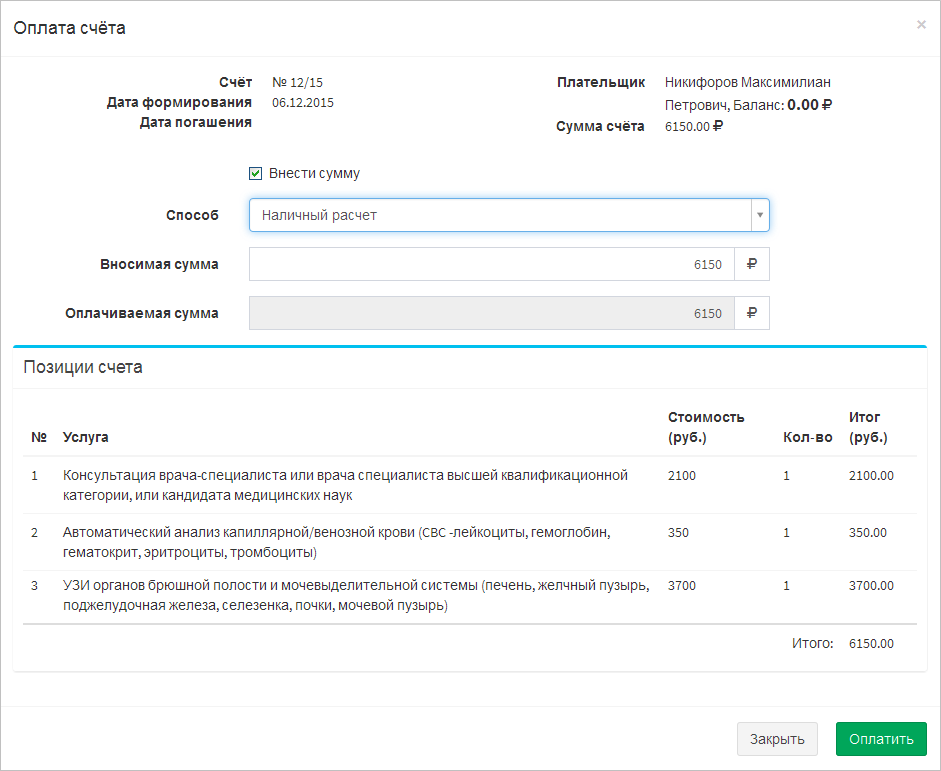
\includegraphics[width = 0.8\textwidth ,keepaspectratio]{kas_payment}
	\caption{Страница <<Оплата счета>>}
	\label{img_kas_payment}
\end{figure}

Для оплаты счета необходимо в центральной части всплавающего окна выбрать тип оплаты в поле \dm{Способ}, указать сумму оплаты в поле \dm{Вносимая сумма} и нажать кнопку \btn{Оплатить} в правом нижнем углу окна. Всплывающее окно будет закрыто, а в списке счетов появится отметка об оплате данного счета.


\subsection{Ведение договоров на оказание платных медицинских услуг}

\subsubsection{Регистрация договоров}

Для создания и просмотра договоров на оплату медицинских услуг, зарегистрированных в системе, необходимо на рабочем столе кассира щелкнуть по плитке \dm{Список договоров}. На открывшейся странице (Рисунок \ref{img_kas_doglist}) появится список договоров, зарегистрированных в \tmisp.

\begin{figure}[ht]\centering
	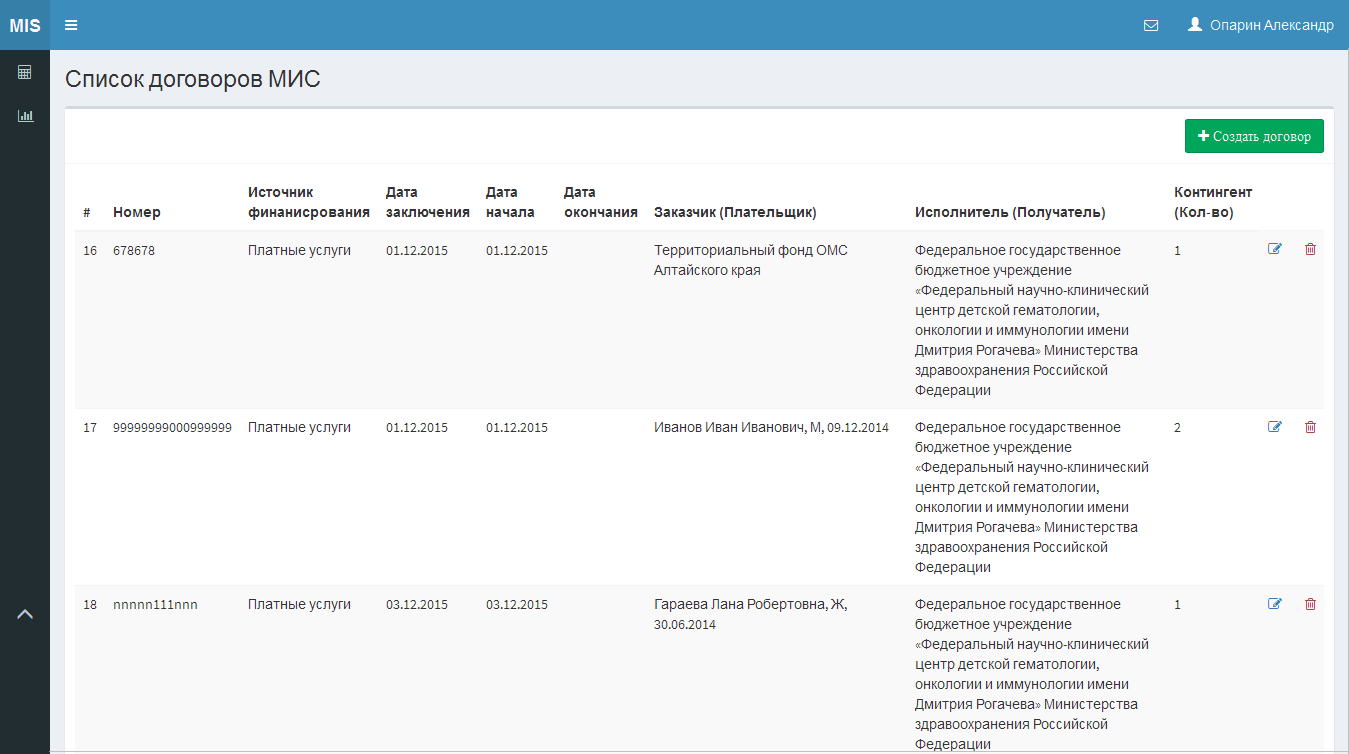
\includegraphics[width = 1\textwidth ,keepaspectratio]{kas_doglist}
	\caption{Страница <<Список договоров>>}
	\label{img_kas_doglist}
\end{figure}

В списке указываются следующие данные:
\begin{itemize}
 \item Номер строки по порядку;
 \item \dm{Номер} -- номер договора;
 \item \dm{Источник финансирования} -- источник финансирования, по которому заключается договор;
 \item \dm{Дата заключения} договора;
 \item \dm{Дата начала} -- дата начала действия договора;
 \item \dm{Дата окончания} -- дата окончания действия договора;
 \item \dm{Заказчик(Плательщик)} -- для плательщиков-физических лиц указываются фамилия, имя, отчество, дата рождения плательщика; для плательщиков-юридических лиц -- наименование организации;
 \item \dm{Исполнитель(Получатель)} -- наименование организации-получателя платежа.
 \item \dm{Контингент (количество)} -- количество пациентов, которые могут обслуживаться по данному договору.
\end{itemize}

Список договоров может размещаться на нескольких страницах. Для перемещения по страницам рекомендуется воспользоваться кнопками навигации, расположенными внизу списка, в правой части каждой страницы.

Для создания нового договора нужно нажать кнопку \btn{$+$ Создать договор} в правом верхнем углу страницы. В появившемся всплывающем окне (Рисунок \ref{img_kas_newdog}) откроется карточка нового договора.
 
\begin{figure}[!ht]\centering
	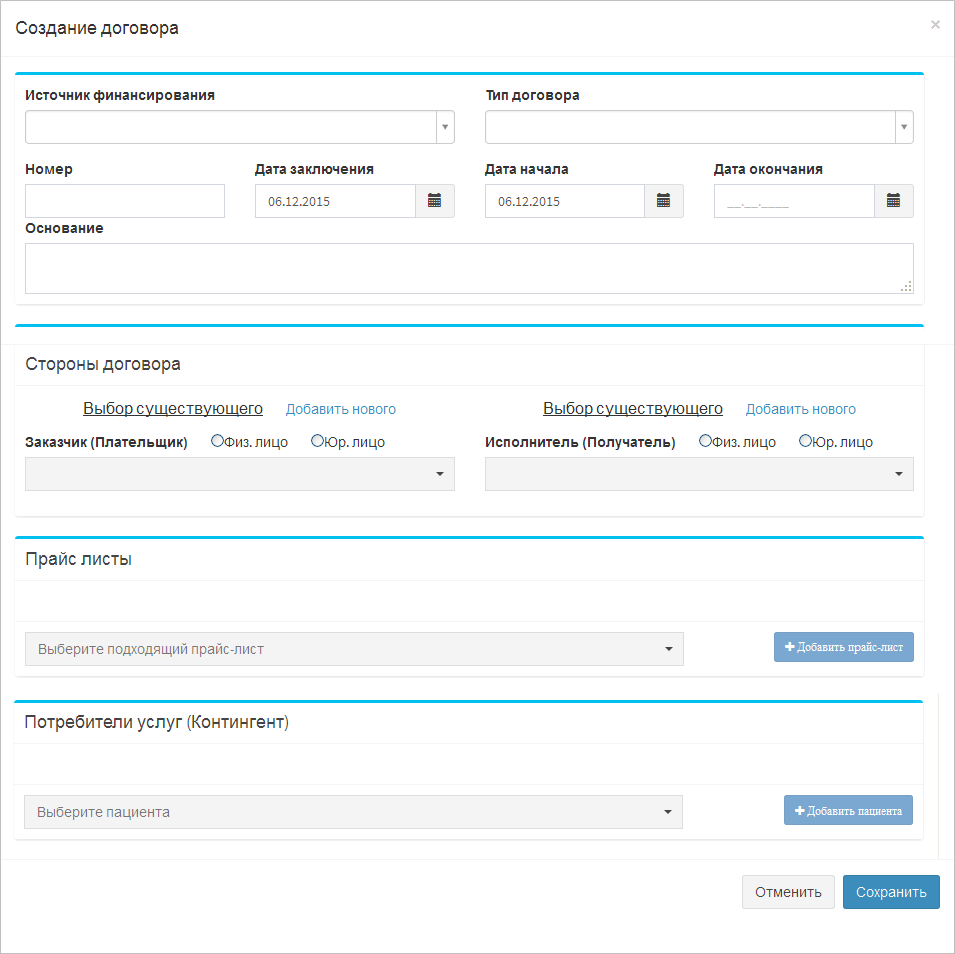
\includegraphics[width = 0.8\textwidth ,keepaspectratio]{kas_newdog}
	\caption{Страница <<Крточка договора>>}
	\label{img_kas_newdog}
\end{figure}

Карточка разделена на несколько блоков:
\begin{enumerate}
 \item Блок \dm{Общая информация} содержит основные сведения о договоре:
 \begin{itemize}
  \item \dm{Источник финансирования} -- выбирается из раскрывающегося списка;
  \item \dm{Тип договора} -- выбирается из раскрывающегося списка;
  \item \dm{Номер} -- регистрационный номер договора;
  \item \dm{Дата заключения} -- дата заключения договора;
  \item \dm{Дата начала} -- дата начала действия договора, может быть больше даты заключения;
  \item \dm{Дата окончания} -- дата окончания действия договора. Если дата окончания не указана, то договор считается бессрочным.
  \item \dm{Основание} -- основание договора, вводится с клавиатуры.
 \end{itemize}
 Все поля, кроме \dm{Дата окончания} и \dm{Основание} являются обязательными для заполнения.
 
 \item Блок \dm{Стороны договора} позволяет указать имена плательщика и получателя договора. В левой части выбирается плательщик, в правой -- получатель. Если плательщик$\slash$получатель  соответственно был ранее зарегистрирован в \tmisp~в качестве участника договора, то следует использовать ссылку <<Выбор существующего>> (выбрано по умолчанию). Поиск при этом будет осуществляться из списка ранее зарегистрированных участников договоров. Если в качестве участника договора он регистрируется впервые, то необходимо щелкнуть по ссылке <<Добавить нового>>, а затем выполнить поиск по фамилии (для физического лица) или наименованию организации (для юридического лица). При этом участник-физическое лицо должен быть предварительно зарегистрирован в системе в качестве пациента, а юридическое лицо -- в справочнике организаций. Установка флажка \dm{Физ.лицо} или \dm{Юр.лицо} ограничивает область поиска выбранным типом участников.
 Поиск осуществляется автоматически по мере ввода имени участника в поле \dm{Заказчик (Плательщик)} или \dm{Исполнитель (Получатель)} соответственно.
 
 \item В блоке \dm{Прайс листы} требуется выбрать из раскрывающегося списка прайс-лист, согласно которому будет осуществлятьса расчет стоимости медицинских услуг по данному договору. По мере ввода текста в поле выбора прайс-листа осуществляется фильтрация доступных в системе прайс-листов по наименованию согласно введенному тексту.
 
 \item В блоке \dm{Потребители услуг (Контингент)} можно указать одного или нескольких пациентов, для которых действителен данный договор. Для добавления пациента необходимо ввести его фамилию в свободное поле в данном блоке. После того как список пациентов будет отфильтрован по фамилии, необходимо выбрать нужную запись из раскрывшегося списка.
 
 Для добавления второго и последующих пациентов в список следует нажать кнопку \btn{$+$ Добавить пациента} в правой части блока и во вновь появившемся поле найти и добавить пациента.
 
 Добавление пациента в данный блок возможно только если он зарегистрирован в картотеке пациентов \tmisr.
\end{enumerate}

\subsubsection{Редактирование договоров}

Открытие ранее созданного договора на редактирование осуществляется нажатием на пиктограмму 
\includegraphics[scale=1]{edt_} справа от соответствующей записи в списке договоров. Будет открыта карточка договора (Рисунок \ref{img_kas_newdog}) заполненными полями. Необходимо внести изменения в даннве договора и нажать кнопку \btn{Сохранить} в правом нижнем углу всплывающего окна.

Для удаления договора из системы необходимо щелкнуть левой кнопкой мыши по пиктограмме 
\includegraphics[scale=1]{del} и во всплывающем окне подтвердить удаление договора, нажав кнопку \btn{Да}. 

